\documentclass[a4paper,11pt]{article}
\usepackage{amsmath,amsthm,amsfonts,amssymb,amscd,amstext,vmargin,graphics,graphicx,tabularx,multicol} 
\usepackage[francais]{babel}
\usepackage[utf8]{inputenc}  
\usepackage[T1]{fontenc} 
\usepackage{pstricks-add,tikz,tkz-tab,variations}
\usepackage[autolanguage,np]{numprint} 

\setmarginsrb{1.5cm}{0.5cm}{1cm}{0.5cm}{0cm}{0cm}{0cm}{0cm} %Gauche, haut, droite, haut
\newcounter{numexo}
\newcommand{\exo}[1]{\stepcounter{numexo}\noindent{\bf Exercice~\thenumexo} : \marginpar{\hfill /#1}}
\reversemarginpar


\newcounter{enumtabi}
\newcounter{enumtaba}
\newcommand{\q}{\stepcounter{enumtabi} \theenumtabi.  }
\newcommand{\qa}{\stepcounter{enumtaba} (\alph{enumtaba}) }
\newcommand{\initq}{\setcounter{enumtabi}{0}}
\newcommand{\initqa}{\setcounter{enumtaba}{0}}

\newcommand{\be}{\begin{enumerate}}
\newcommand{\ee}{\end{enumerate}}
\newcommand{\bi}{\begin{itemize}}
\newcommand{\ei}{\end{itemize}}
\newcommand{\bp}{\begin{pspicture*}}
\newcommand{\ep}{\end{pspicture*}}
\newcommand{\bt}{\begin{tabular}}
\newcommand{\et}{\end{tabular}}
\renewcommand{\tabularxcolumn}[1]{>{\centering}m{#1}} %(colonne m{} centrée, au lieu de p par défault) 
\newcommand{\tnl}{\tabularnewline}

\newcommand{\trait}{\noindent \rule{\linewidth}{0.2mm}}
\newcommand{\hs}[1]{\hspace{#1}}
\newcommand{\vs}[1]{\vspace{#1}}

\newcommand{\N}{\mathbb{N}}
\newcommand{\Z}{\mathbb{Z}}
\newcommand{\R}{\mathbb{R}}
\newcommand{\C}{\mathbb{C}}
\newcommand{\Dcal}{\mathcal{D}}
\newcommand{\Ccal}{\mathcal{C}}
\newcommand{\mc}{\mathcal}

\newcommand{\vect}[1]{\overrightarrow{#1}}
\newcommand{\ds}{\displaystyle}
\newcommand{\eq}{\quad \Leftrightarrow \quad}
\newcommand{\vecti}{\vec{\imath}}
\newcommand{\vectj}{\vec{\jmath}}
\newcommand{\Oij}{(O;\vec{\imath}, \vec{\jmath})}
\newcommand{\OIJ}{(O;I,J)}


\newcommand{\bmul}[1]{\begin{multicols}{#1}}
\newcommand{\emul}{\end{multicols}}

\newcommand{\reponse}[1][1]{%
\multido{}{#1}{\makebox[\linewidth]{\rule[0pt]{0pt}{20pt}\dotfill}
}}

\newcommand{\titre}[5] 
% #1: titre #2: haut gauche #3: bas gauche #4: haut droite #5: bas droite
{
\noindent #2 \hfill #4 \\
#3 \hfill #5

\vspace{-1.6cm}

\begin{center}\rule{6cm}{0.5mm}\end{center}
\vspace{0.2cm}
\begin{center}{\large{\textbf{#1}}}\end{center}
\begin{center}\rule{6cm}{0.5mm}\end{center}
}



\begin{document}
\pagestyle{empty}
\titre{Contrôle 2}{Nom :}{Prénom :}{Classe}{Date}



\exo{4} Donner les résultats sous forme de \textbf{fraction irréductible}  \\

\bmul{3}

 $T = \dfrac{45}{28} \times \dfrac{7}{9} $

\columnbreak

 $B = \dfrac{\dfrac{5}{4}}{\dfrac{-15}{8}}$

\columnbreak

 $I=(\dfrac{3}{8} + \dfrac{1}{4}) \div (\dfrac{4}{3} - \dfrac{1}{6}) $
 
\emul

\exo{2} Vrai ou Faux\\

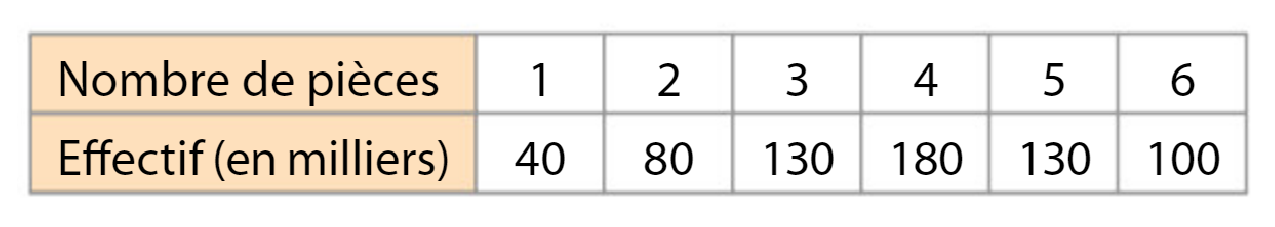
\includegraphics[scale=1]{tab.eps} \\


\exo{4} Proportionnalité\\

\q \begin{center}
\begin{tabular}{|c|c|c|c|c|}
\hline 
Quantité de poires (en kg) & 3 & 5 & 8 & 6 \\ 
\hline 
Prix (en euros) & 6,45 & 10,75 & 17,20 & 12,90 \\ 
\hline 
\end{tabular}\\
\end{center}

  Le prix des poires est-il proportionnel à leur quantité ? \textbf{Justifier votre réponse.}\\

\q \begin{center}
\begin{tabular}{|c|c|c|c|c|}
\hline 
Nombre de DVD & 2 & 4 & 6 & 8 \\ 
\hline 
Prix (en euros) & 7,50 & 14 & 19 & 24 \\ 
\hline 
\end{tabular} 
\end{center}

Voici des tarifs de location de DVD proposés sur internet. Y a-t-il proportionnalité entre le prix et le nombre de DVD ?\\

\q Compléter le tableau de proportionnalité suivant :\\

\begin{center}
\begin{tabular}{|c|c|c|c|c|c|}
\hline 
Prix (en euros) & 15 & 45,65 & 123,90 &  &  \\ 
\hline 
Prix (en dollars) & 16,5 &  &  & 50,40 & 32 \\ 
\hline 
\end{tabular} \\
\end{center}

\q Il faut 8 arrosoir pour remplir un bac de 50 litres. Combien faut-il d'arrosoir pour remplir une cuve de 225 litres ? une cuve de 300 litres ?\\

\exo{1,5} Pourcentage \\

Dans un stade, il y a 16 000 spectateurs. 10 000 supportent l'équipe locale et 6 000 l'équipe adverse. Parmi les supporteurs de l'équipe locale, il y a 80$\%$ de garçons et parmi les supporteurs de l'équipe adverse, il y a 60 $\%$ de garçons.\\
Quel est le pourcentage de garçons dans le stade?\\

\newpage

\exo{2,5}

\bmul{2}


\includegraphics[scale=1]{tsunami.eps} 
\columnbreak

L'explosion d'un volcan, situé en mer, provoque la formation d'un raz de marée ou "tsunami" : formidable vaque de plusieurs dizaines de mètres de hauteur se déplaçant à la vitesse de 138,89 m/s.
\emul

\noindent \initq \q Transformer cette vitesse pour l'obtenir en km/h.\\
\q En combien de temps la vague va-t-elle atteindre la maison?\\
\q Quelle distance aura parcouru la vague en 1 min puis en 45 min ?\\


\exo{4}


 \bmul{2}
\initq \q On considère un triangle ABC. M est un point de [AB], N un point de [AC] et les droites (MN) et (BC) sont parallèles.
D'après le théorème de Thalès, on a :\\

$.......... = ............. = ..............$\\

\columnbreak
\begin{center}

\includegraphics[scale=1]{thales.eps} 
\end{center}
\emul 

\bmul{2}
\q Les droites (BC) et (MN) sont parallèles.\\
Calcule AN et AB.

\columnbreak


\includegraphics[scale=1]{thalesbis.eps} 

\emul

\exo{2}

\bmul{2}
Une personne observe une éclipse de soleil.\\
Cette situation est schématisée par le dessin ci-contre.\\
L'observateur est en T. Les points S (centre du soleil), L(centre de la lune) et T sont alignés.\\
Le rayon SO du soleil mesure 695 000 km.\\
Le rayon LU de la lune mesure 1 736 km.\\
La distance TS est 150 millions de km.\\
Calculer la distance TL (on donnera l'arrondi au km).\\

\columnbreak

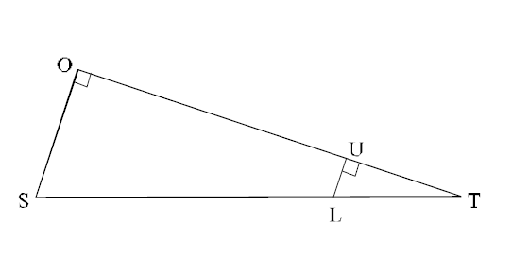
\includegraphics[scale=1]{thalestrois.eps} 

\emul


\end{document}
